\chapter{Preliminary}

As the target platform for this work is the graph database neo4J, we will mostly consider \textit{directed} graphs. From the terminology we always refer \textit{arcs}, which is an directed edge.
In some cases we will refer to \textit{edges}, in these cases the direction doesn't play a role.

\section{Notation and Expressions}
We denote a graph $G(V, A)$ in case me mean an \textit{directed} graph, where $v$ is a vertex contained in the vertices $v \epsilon  V$ and $a$ is an
arc $a \epsilon A$. An arc is uniquely defined by to vertices $v_a$ and $v_b$ such that $v_a \neq v_b$, so there are no loops nor multi edges.
An edge additionally has a weight function $w: A \rightarrow \mathbb{R}_{<0} $ it's weight which must be a positive.
\\
We use $A$ as the arc set and $a$ a single arc which is directed. $a \epsilon A$ can be replace with $e \epsilon E$ which refers to edges that are \textit{undirected}. 
\\
$G$ represents the input graph. The contraction graph $G'(V', A')$ is the graph that will be used at contraction for initially building the CCH index structure. A vertex $v$ in will 
never be really deleted. Instead the rank property $r(v)$ is set to mark this as an already contracted. So $V \equiv V'$ but $A \subseteq A'$ there will be edges add while building
the CCH index. $S = A' \setminus A$ is the shortcut set that is added throughout the contraction. 
\\
$G^*(V^*, A^*)$ is the is the search graph while doing one a shortest path query. Futhermore one query will have two search graphs. $G^*_\uparrow$ representing the upwards search graph
and the $G^*_\downarrow$.
\\
Finally there will be the edge set of edges that are written to the disk. These will $\bigcirc A$ will be separated into to sets $\bigcirc A_\downarrow$ and $\bigcirc A_\uparrow $, too. 

\section{Updating Priority Queue}

One data structure that is heavily used in this paper is a priority queue. This a very useful structure as it returns always the element with the lowest priority. In dijkstras algorithm for example, the
priority is calculated on the weight, so by retrieving an vertex you will always get the next shortest path. 
The problem arises when it comes to updating an element of an priority queue that is already in the queue, because a priority queue can holt the same element multiple times and even with the different priorities. 
This explanation refers to the \cite[Java 17 reference]{JavaPrioQueue}, but priority queues are which based an a \cite[binary heap]{floyd1964algorithm} as this one should have all the same properties. \\
One might ask why can't we simply remove the element that is already in the queue and then re-push it. That is actually possible but slow, as the operations \textit{contains(element), and remove(element)} are running in linear time $\mathcal{O}(n) $. Better would be to use 
\textit{offer(), poll(), remove() or add()} which run in logarithmic time $\mathcal{O}( \log (n))$. 
One could think of just keeping a reference to the element and later on change the priority as needed. But the queue will not be notified buy such a manipulation, and because queue keeps the next element to dequeue at 
the top one will retrieve the wrong element. So we have to cum up with something better.
If the priority of an element can only decrease, this usually doesn't cause a problem, because by retrieving an element you will definitely get the one with the lowest priority. Therefore you can simply repush elements
to the queue, as you will always get the real smallest possible. To avoid processing an element twice you insert the elements into a set where you keep track of the already processed onces and if you retrieve a already seen
one you simply pull again. 
If the priority can decrease and increase and you simply push updated the elements to again, the problem is a bit more difficult as now you can possibly dequeue an element with the old priority which is lower as the current but not valid anymore.
We initialize a priority queue and a map which key is the element and the value is a integer a version number. If we push an element to the queue we check whether the element is already in the control map, if not not we insert it together with the value $0$. 
Then we wrap the element together with the $0$ and insert it into the queue. If the element is already in the control mal we increase the value it has in the map by one, wrap this new version number together with the element and push it queue. 
At pull we retrieve the element together with its current version number. If the number is not equal to the one in the control map we simply pull again and check again until we find an element that is up to date.


\section{Dijkstra}

We want to do a little recap on dijkstras algorithm as it crucial for the ch/cch search. Additionally we want to decuple two thing that are usually done together. The initialization of a dijkstra query and
the iteration step, that expands vertices until the shortest path to the target is found. Looking at algorithm \ref{alg:disjkstra_algorithm} the \textit{expandNext()} procedure is what usually done in a
while loop until the \textit{isComplete()} function returns \textit{true} and all requested shortest paths are found or all vertices have been expanded. We provide this with the function \textit{getResult()} 
on such a dijkstra query object as you can see in figure \ref{fig:dijkstra_class}. Being able to call the \textit{expandNext()} procedure from outside is a very powerful. For example if we want to write a bidirectional
dijkstra, we can create to two instances of the class \textit{Dijkstra} as stated in figure \ref{fig:dijkstra_class}. One dijkstra is initialized only with outgoing 
$\text{Dijkstra(}s, [t,], \overrightarrow{G}(V, \overrightarrow{A}) \text{)}$ arcs the other only with incoming arcs $\text{Dijkstra(}t, [s], \overleftarrow{G}(V, \overleftarrow{A}) \text{)}$. Now we can build our 
algorithm around that tell the bidirectional query when to stop or which side to expand next, but the essential thing here is we have reused the logic of the \textit{expandNext()} procedure and not written it again.

\begin{frame}
    \frametitle{Dijkstra}
    Let's go from $v_2$ to $v_3$
    \vfill
    \begin{columns}
    \column{0.5\textwidth}
    \centering
    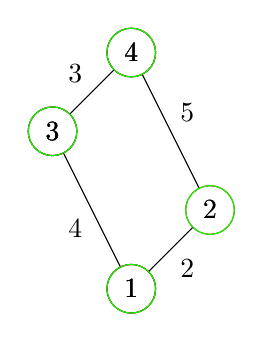
\begin{tikzpicture}[node distance={15mm}, main/.style = {draw, circle}]
        
        \onslide<1-2>{\node[main] (x3) at (0, 2) {$3$};}
        \onslide<3-4>{\node[main, draw=red] (x3) at (0, 2) {$3$};}
        \onslide<5->{\node[main, draw=green] (x3) at (0, 2) {$3$};}
        \onslide<1>{\node[main] (x4) at (1, 3) {$4$};}
        \onslide<2-3>{\node[main, draw=red] (x4) at (1, 3) {$4$};}
        \onslide<4->{\node[main, draw=green] (x4) at (1, 3) {$4$};}
        \onslide<1>{\node[main, draw=red] (x2) at (2, 1) {$2$};}
        \onslide<2->{\node[main, draw=green] (x2) at (2, 1) {$  2$};}
        \onslide<1>{\node[main] (x1) at (1, 0) {$1$};}
        \onslide<2>{\node[main, draw=red] (x1) at (1, 0) {$1$};}
        \onslide<3->{\node[main, draw=green] (x1) at (1, 0) {$1$};}
        
        \draw (x1) -- node[below right] {$2$}(x2);
        \draw (x1) -- node[below left] {$4$} (x3);
        \draw (x2) -- node[above right] {$5$} (x4);
        \draw (x3) -- node[above left] {$3$} (x4);

    \end{tikzpicture}
    \column{0.5\textwidth}
    \centering
    \begin{tabular}{c | c | c}
        \textbf{id} & \textbf{dist} & \textbf{settled}\\
        \hline 
        2 & 0  & \onslide<1>{false} \onslide<2->{true} \\ 
        \hline \pause
        1 & 2 & \onslide<2>{false} \onslide<3->{true}\\ 
        \hline
        4 &  5 & \onslide<2-3>{false} \onslide<4->{true} \\
        \hline \pause
        3 & 6 & \onslide<3-4>{false} \onslide<5->{true}\\ 
    \end{tabular}
\end{columns}
          
    

\end{frame}


\begin{figure}
    \centering
    \begin{frame}
    \frametitle{Dijkstra}
    Let's go from $v_2$ to $v_3$
    \vfill
    \begin{columns}
    \column{0.5\textwidth}
    \centering
    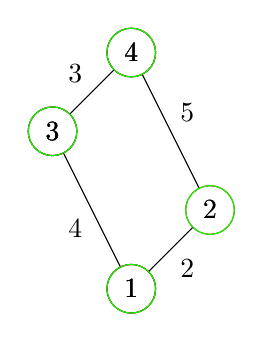
\begin{tikzpicture}[node distance={15mm}, main/.style = {draw, circle}]
        
        \onslide<1-2>{\node[main] (x3) at (0, 2) {$3$};}
        \onslide<3-4>{\node[main, draw=red] (x3) at (0, 2) {$3$};}
        \onslide<5->{\node[main, draw=green] (x3) at (0, 2) {$3$};}
        \onslide<1>{\node[main] (x4) at (1, 3) {$4$};}
        \onslide<2-3>{\node[main, draw=red] (x4) at (1, 3) {$4$};}
        \onslide<4->{\node[main, draw=green] (x4) at (1, 3) {$4$};}
        \onslide<1>{\node[main, draw=red] (x2) at (2, 1) {$2$};}
        \onslide<2->{\node[main, draw=green] (x2) at (2, 1) {$  2$};}
        \onslide<1>{\node[main] (x1) at (1, 0) {$1$};}
        \onslide<2>{\node[main, draw=red] (x1) at (1, 0) {$1$};}
        \onslide<3->{\node[main, draw=green] (x1) at (1, 0) {$1$};}
        
        \draw (x1) -- node[below right] {$2$}(x2);
        \draw (x1) -- node[below left] {$4$} (x3);
        \draw (x2) -- node[above right] {$5$} (x4);
        \draw (x3) -- node[above left] {$3$} (x4);

    \end{tikzpicture}
    \column{0.5\textwidth}
    \centering
    \begin{tabular}{c | c | c}
        \textbf{id} & \textbf{dist} & \textbf{settled}\\
        \hline 
        2 & 0  & \onslide<1>{false} \onslide<2->{true} \\ 
        \hline \pause
        1 & 2 & \onslide<2>{false} \onslide<3->{true}\\ 
        \hline
        4 &  5 & \onslide<2-3>{false} \onslide<4->{true} \\
        \hline \pause
        3 & 6 & \onslide<3-4>{false} \onslide<5->{true}\\ 
    \end{tabular}
\end{columns}
          
    

\end{frame}
    \caption{Dijkstra Class Diagram}
    \label{fig:dijkstra_class}
\end{figure}


